\documentclass[handout]{beamer}
%\documentclass{beamer}
\usepackage{pgfpages}
\usepackage{eurosym}
\setbeamertemplate{footline}[frame number]
%\pgfpagesuselayout{2 on 1}[a4paper,portrait,border shrink=5mm]
\usetheme{Copenhagen} % Beamer Theme
\usecolortheme{crane_unibw} % BeamerColor Theme
%\useoutertheme[subsection=false]{smoothbars} % Beamer Outer Theme
\setbeamertemplate{blocks}[rounded][shadow=true]
%\useoutertheme{infolines}
%\useinnertheme{rectangles}
\setbeamercovered{transparent}
%\usepackage{beamerthemeshadow}
\usepackage[latin9]{inputenc}
\usepackage{graphicx}
\usepackage[british,ngerman]{babel}
\usepackage{curves}
\usepackage{epic}
\usepackage{setspace}
\usepackage{amsmath,amssymb,dsfont,stmaryrd}
\usepackage{pgfpages}
\usepackage{hyperref}
%\usepackage{xspace}
\newcommand{\C}[1]{% stellt Buchstaben als script letter \mathcal{} dar
\ensuremath{\mathcal{#1}}\xspace}

\newcommand{\D}[1]{% stellt Buchstaben als script letter \mathds{} dar
\ensuremath{\mathds{#1}}\xspace}

\newcommand{\B}[1]{% stellt Buchstaben als script letter \mathbb{}  dar
\ensuremath{\mathbb{#1}}\xspace}

\newcommand{\F}[1]{% stellt Buchstaben als Frakturschrift dar
\ensuremath{\mathfrak{#1}}\xspace}

\newcommand{\Bf}[1]{% stellt Buchstaben im Mathemodus fett  \mathbf{}  dar
\ensuremath{\mathbf{#1}}\xspace}


\newcommand{\Z}[1]{%
\ensuremath{\mathscr{#1}}\xspace}


\newcommand{\FC}[0]{% 
\ensuremath{\mathfrak{C}}\xspace}
\newcommand{\CT}[0]{% 
\ensuremath{\mathcal{T}}\xspace}
\newcommand{\CB}[0]{% 
\ensuremath{\mathcal{B}}\xspace}


\newcommand{\FO}[0]{%
\ensuremath{\mathfrak{O}}\xspace}

\newcommand{\fett}[1]{{\bf #1}}

\newcommand{\OL}[1]{%
\ensuremath{\overline{#1}}\xspace}

\definecolor{darkblue}{rgb}{0,0,.5}
\hypersetup{pdftex=true, colorlinks=true, breaklinks=true,
  linkcolor=darkblue, menucolor=darkblue,
 pagecolor=darkblue, urlcolor=darkblue}
%\pgfpagesuselayout{4 on 1}[a4paper,landscape,border shrink=5mm]

%% FrameNr setzen (links unten) Frame / FrameGes.
\setbeamertemplate{footline}{%
\begin{beamercolorbox}[wd=\paperwidth,ht=2.25ex,dp=1ex]{date in
head/foot}%
\hfill \insertframenumber{} / \inserttotalframenumber \hspace*{1ex} 
% 
\end{beamercolorbox}}%
\usepackage{xspace}
\newcommand{\C}[1]{% stellt Buchstaben als script letter \mathcal{} dar
\ensuremath{\mathcal{#1}}\xspace}

\newcommand{\D}[1]{% stellt Buchstaben als script letter \mathds{} dar
\ensuremath{\mathds{#1}}\xspace}

\newcommand{\B}[1]{% stellt Buchstaben als script letter \mathbb{}  dar
\ensuremath{\mathbb{#1}}\xspace}

\newcommand{\F}[1]{% stellt Buchstaben als Frakturschrift dar
\ensuremath{\mathfrak{#1}}\xspace}

\newcommand{\Bf}[1]{% stellt Buchstaben im Mathemodus fett  \mathbf{}  dar
\ensuremath{\mathbf{#1}}\xspace}


\newcommand{\Z}[1]{%
\ensuremath{\mathscr{#1}}\xspace}


\newcommand{\FC}[0]{% 
\ensuremath{\mathfrak{C}}\xspace}
\newcommand{\CT}[0]{% 
\ensuremath{\mathcal{T}}\xspace}
\newcommand{\CB}[0]{% 
\ensuremath{\mathcal{B}}\xspace}


\newcommand{\FO}[0]{%
\ensuremath{\mathfrak{O}}\xspace}

\newcommand{\fett}[1]{{\bf #1}}

\newcommand{\OL}[1]{%
\ensuremath{\overline{#1}}\xspace}

\begin{document}
\title{Visualisierung multisensorischer Daten zur Vorbereitung von Datenfusion}
\subtitle{am Beispiel einer milit�rischen Lage}
\author{Stephan Tzschoppe}
\institute[Universit�t der Bundeswehr M�nchen]{Institut f�r Theoretische Informatik, \\
Mathematik und Operations Research \\ 

Fakult�t f�r Informatik \\
}
%\institute[]{Institut für \\ Fakultät für Informatik\\Universität der Bundeswehr München}
\date{18.02.2010}
%%%%%Logo auf jeder Seite%%%%%%%%%%%%%%%%%%%%%%%
\pgfdeclareimage[height=2cm]{bwlogo}{Bilder/UniBwM_logo} \logo{\pgfuseimage{bwlogo}}
%%%%%%%%%%%%%%%%%%%%%%%%%%%%%%%%%%%%%%%%%%%%%%%%
%%%%%%Logo nur auf der Titelseite
%\titlegraphic{\pgfuseimage{bwlogo}}
%%%%%%%%%%%%%%%%%%%%%%%%%%
\begin{frame}
\titlepage
\end{frame}

\begin{frame}
\frametitle{Inhaltsverzeichnis}
\begin{footnotesize}
\tableofcontents
\end{footnotesize}
\end{frame}


\section{Motivation}
\subsection{Milit�rische Lage}
\begin{frame}\frametitle{Lagebeispiel}  

 \begin{columns}[t]
\begin{column}{5cm}
  \begin{block}{2 eigene Panzer (blau)}
    \begin{itemize}[<+-| alert@+>]
  	  \item bewegen sich nicht
  	  \item melden Beobachtungen in konstanten Zeitabst�nden
    \end{itemize}
  \end{block}\end{column}
\begin{column}{5cm}
  \begin{block}{2 feindliche Panzer (rot)}
  \begin{itemize}[<+-| alert@+>]
  	\item ein Panzer in Querfahrt
  	\item ein Panzer in in Richtung der eigenen Kr�fte
    \end{itemize}
\end{block}\end{column}
\end{columns}
\end{frame}

\begin{frame}\frametitle{Darstellung der Beispiellage}
\begin{figure}[h]
	\centering
		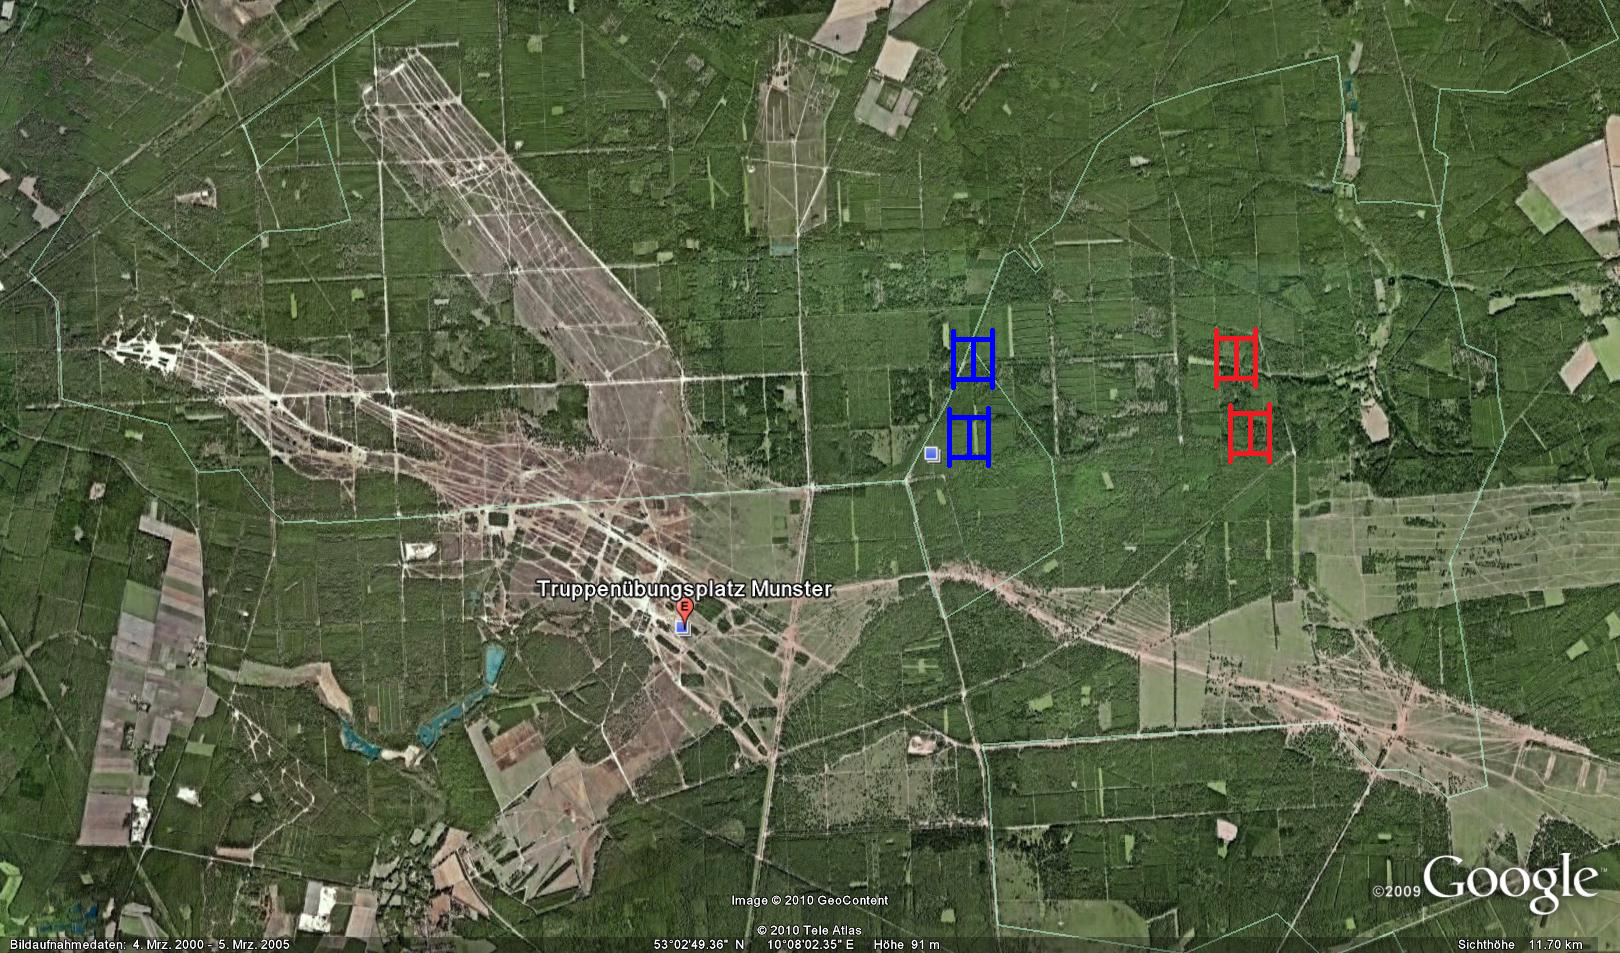
\includegraphics[width=0.80\textwidth]{Bilder/googleearth.png}
	\caption{Lage zum ersten Meldezeitpunkt}
	\label{fig:googleearth}
\end{figure}
\end{frame}

\begin{frame}\frametitle{Darstellung der Beispiellage}
\begin{figure}[h]
	\centering
		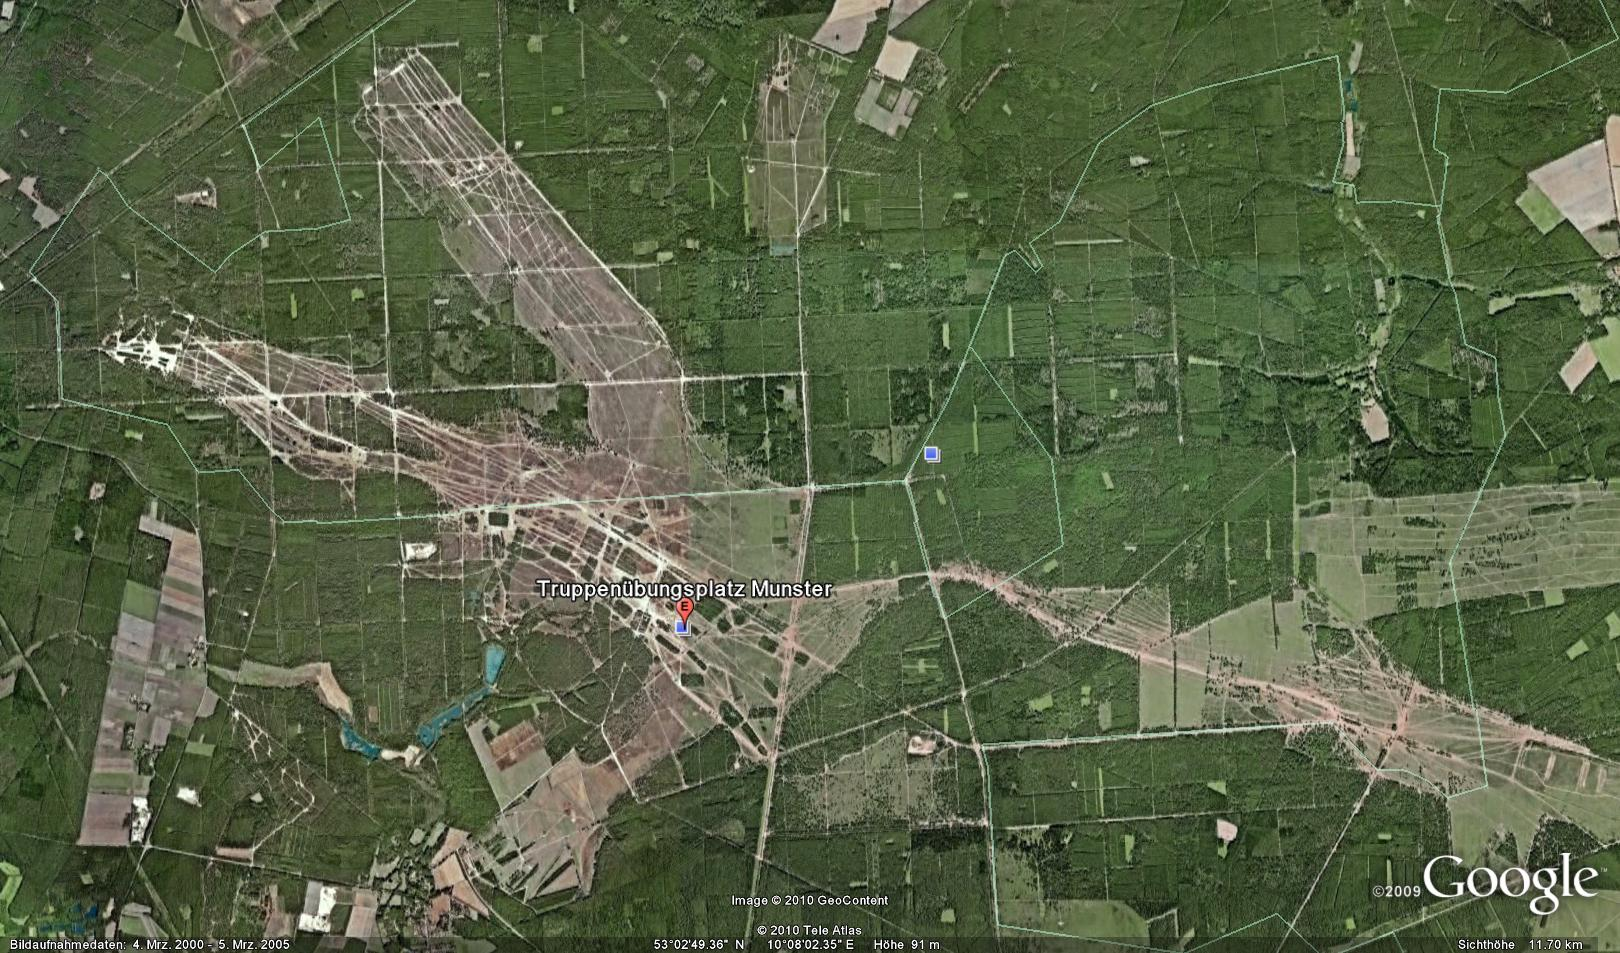
\includegraphics[width=0.80\textwidth]{Bilder/googleearth2.png}
	\caption{Lage zum zweiten Meldezeitpunkt}
	\label{fig:googleearth2}
\end{figure}
\end{frame}

\begin{frame}\frametitle{Darstellung der Beispiellage}
\begin{figure}[h]
	\centering
		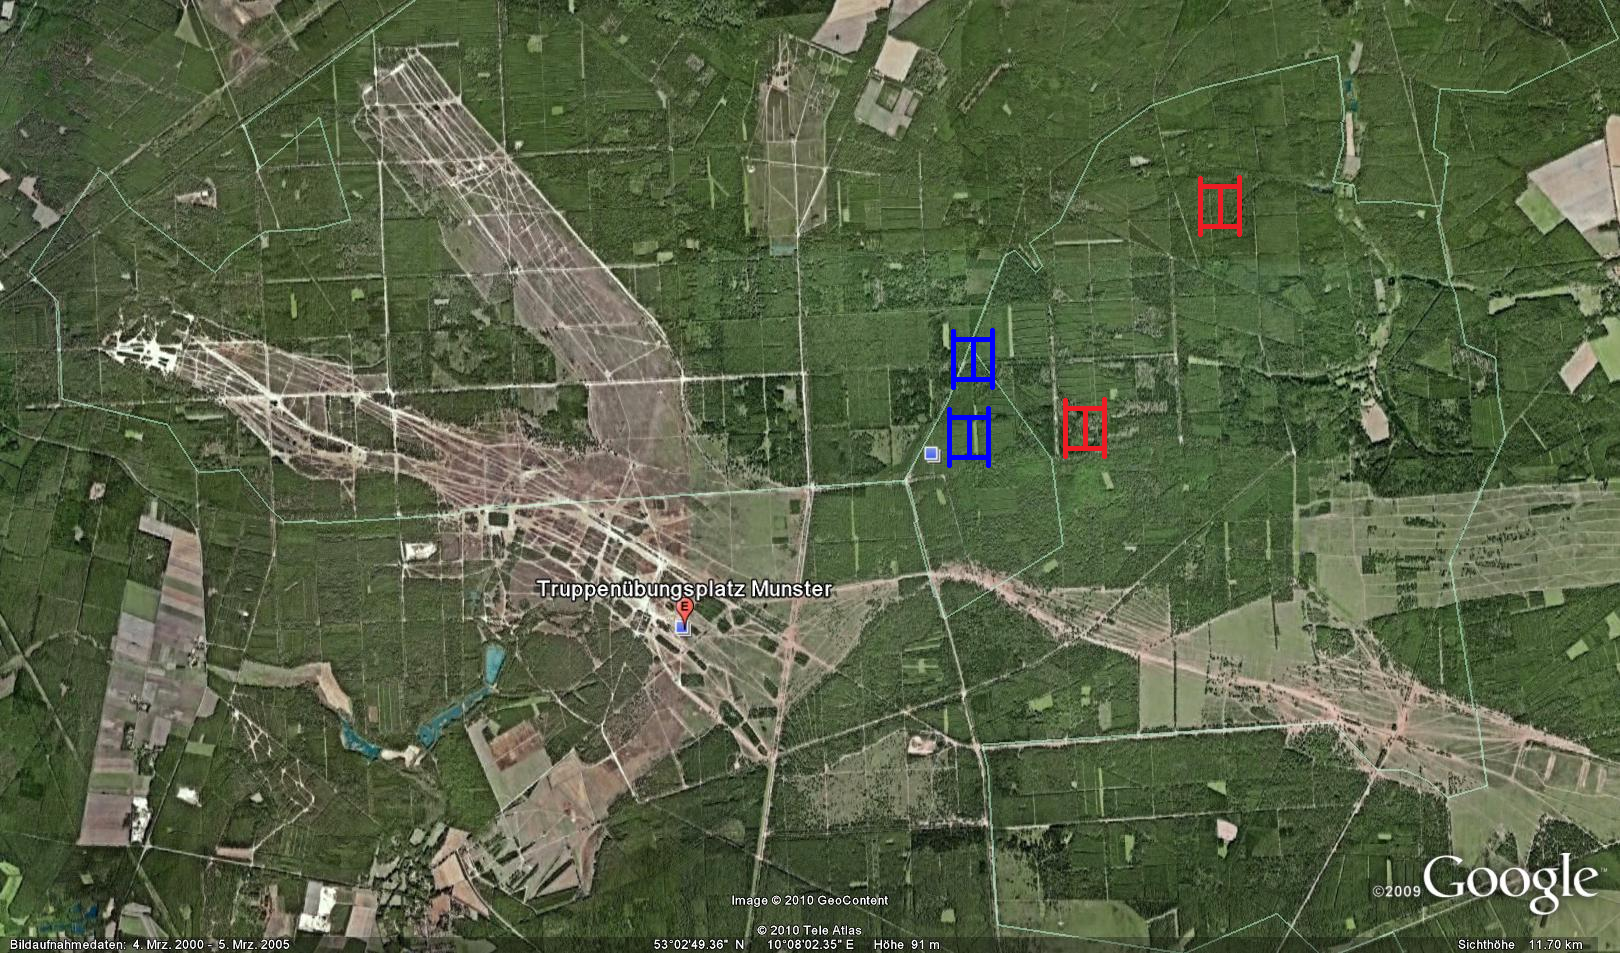
\includegraphics[width=0.80\textwidth]{Bilder/googleearth3.png}
	\caption{Lage zum dritten Meldezeitpunkt}
	\label{fig:googleearth3}
\end{figure}
\end{frame}

\subsection{Repr�sentation der Daten}

\begin{frame}[fragile]
\frametitle{Darstellung der Meldungen in XML}
\lstset{%
language=XML,
basicstyle={\ttfamily \tiny},
numbers=left,                   % where to put the line-numbers
numberstyle=\tiny,      % the size of the fonts that are used for the line-numbers
stepnumber=1
}%
\begin{lstlisting}[breaklines=true,frame=tlRB,captionpos=b,caption={Darstellung einer Meldung in XML}] 
<Situation>
  <Units>
   <Unit>
      <Name>FriendlyTank1</Name>
      <Location>
        <Lat>52.796629714678467</Lat>
        <Lon>9.89990561649954</Lon>
        <LastModified>2009-02-20T10:25:36+01:00</LastModified>
      </Location>
    </Unit>
    <Unit>
      <Name>FriendlyTank2</Name>
      <Location>
        <Lat>52.794038961891268</Lat>
        <Lon>9.9011727699025922</Lon>
        <LastModified>2009-02-20T10:25:36+01:00</LastModified>
      </Location>
    </Unit>
  </Units>
</Situation>
\end{lstlisting}
\end{frame}

\subsection{Problemstellung}

\begin{frame}\frametitle{Problemstellung}

\begin{block}{Redundante Meldungen zu einem Objekt}
\begin{itemize}[<+-| alert@+>]
    \item Sichtung unterschiedlicher Beobachter zur selben Zeit
    \item Sichtung zu unterschiedlichen Zeiten
\end{itemize}
\end{block}
\begin{itemize}[<+-| alert@+>]
    \item Redundanzen verf�lschen die Lage
    \item Weiterverarbeitung und Analyse unm�glich
    \item \textbf{Beseitigung der Redundanzen ist notwendig}
\end{itemize}
\end{frame}


%----------------------------------------------------------------%
% theorie.tex																			       %
%----------------------------------------------------------------%

\chapter{Multisensorische Daten und ihre Visualisierung}
\label{ch:theorie}

In diesem Kapitel soll zuerst der Zusammenhang zwischen dem Thema dieser Arbeit und den daf�r relevanten theoretischen Grundlagen dargelegt werden. Darauf folgend sollen M�glichkeiten der Datenvisualisierung aufgezeigt. Einige davon sind in der prototypischen Implementierung umgesetzt, andere wurden nicht aufgenommen. Die Gr�nde daf�r sollen an geeigneter Stelle dargelegt werden.

\section{Theoretische Einordnung}
\label{sec:TheoretischeEinordnung}
In diesem Abschnitt soll die  theoretische Einordnung der Arbeit erfolgen. An erster Stelle steht dabei die Erl�uterung multisensorischer Daten anhand eines einfachen Beispiels. Anschlie�end soll mit dessen Hilfe der Begriff \emph{Multisensor Data Fusion} definiert und der praktische Teil dieser Arbeit in den theoretischen Kontext eingeordnet werden.

\subsection{Multisensorische Daten}
\label{sec:EigenschaftenVonMultisensorischenDaten}
Der Begriff der \emph{multisensorischen Daten} existiert in der Literatur nicht losgel�st. Interessant ist er nur in Verbindung der Fusion von Daten. Trotzdem soll an dieser Stelle eine kurze begriffliche Betrachtung stehen.

\label{beispiel}
Ein kleines Beispiel verdeutlicht sehr gut, worum es hier geht: Man stelle sich einen Tisch vor, auf dem zwei brennende Kerzen stehen. Davor befinden sich drei Beobachter. Jeder soll unabh�ngig von den anderen jeden Gegenstand, den er sieht, auf je einem Blatt Papier beschreiben. Bei den entstehenden Dokumenten handelt es sich um eine Form von multisensorischen Daten. Ein Datum ist dabei eine Beschreibung eines Gegenstandes. Ein Sensor ist jeweils einer der Beobachter.  Dies ist ein Ansatz, sich der Thematik zu n�hern. 

Ein anderer Ansatz k�nnte bei selbem Aufbau mit einer Person gemacht werden. Denn der Mensch, oder besser seine Sinne liefert schon multisensorische Daten. Die Person sieht eine Lichtquelle und f�hlt eine Hitzequelle. Diese beiden Beobachtungen sind die Daten, die Sensoren sind Tastsinn und Sehsinn.

Multisensorische Daten wie oben geschildert sind aber in der Theorie und Praxis nicht von Bedeutung, wenn sie f�r sich genommen werden. Schl�ssige Informationen daraus sind n�mlich nicht m�glich, ohne die Eingangsdaten zu interpretieren. Dieser Vorgang, man spricht von \emph{Multisensor Data Fusion}, soll in Abschnitt \ref{sec:MultisensorFusion} erl�utert werden.
\paragraph{Vorteile}
\label{sec:Vorteile}
In \cite{MDFLLINAS} werden neun Vorteile von multisensorischen Systemen (und den von ihnen gelieferten Daten) aufgez�hlt, die hier in Auswahl sinngem�� wiedergegeben werden sollen:

\begin{enumerate}
	\item \textbf{Robustheit:} Informationen k�nnen weiter gesammelt werden, auch wenn ein oder mehrere Sensoren keine Daten mehr liefern.

	\item \textbf{R\protect\"aumlich weitreichende Abdeckung:} Daten, die vielleicht nur von einem ein paar Sensoren gesehen werden, w�rden nicht entdeckt, wenn nur ein einzelner Sensor an der falschen Stelle steht.

	\item \textbf{Zeitlich weitreichende Abdeckung:} Nicht jeder Sensor steht zu jeder Zeit zur Verf�gung. Bei zeitlichem Versatz und �berlappung kann eine dauerhafte Datensammlung betrieben werden.

	\item \textbf{Gesteigerte Informationssicherheit:} Wird ein Datum durch mehrere Sensoren erfasst, verringert sich die Wahrscheinlichkeit eines Messfehlers.

	\item \textbf{Erh�hte Informationsdichte:} Die Aufl�sung, mit der mehrer Sensoren ein Gebiet abtasten k�nnen, ist h�her als die Aufl�sung eines einzelnen Sensors.
\end{enumerate}

Diese Reihe von Vorteilen zeigt, dass die Datensammlung mit mehreren Sensoren durchaus betrieben werden sollte. Die entstehenden Daten bieten vor allem durch ihre Redundanzen  mehr und sichere Informationen als die eines einzelnen Sensors.

\paragraph{Nachteile}
\label{sec:Nachteile}
Die oben angesprochene Redundanz ist zugleich der gr��te Nachteil von multisensorischen Daten. Wie sich das �u�ert, sei noch mal an dem in Abschnitt \ref{beispiel} eingef�hrten Beispiel erl�utert: Die schriftlich gesammelten Daten der drei Beobachter werden an eine Person weitergegeben, die sich zum Zeitpunkt der Beobachtungen an einem anderen Ort aufhielt. Diese Person soll aus den Daten schlie�en, was sich auf dem Tisch befand. Sie hat dabei keine Informationen, welche Daten von welchem Beobachter stammen. Ebenfalls ist unbekannt, wie viele Beobachter �berhaupt beteiligt waren.

Aus den Daten k�nnte die auswertende Person schlie�en, dass sechs Kerzen auf dem Tisch befanden. Dies ist ein v�llig falsches Bild und der Grund f�r die Fehlinterpretation ist die Redundanz der Daten, die nicht beseitigt wurde. Nur wenn Datens�tze, die zu einem realen Objekt geh�ren, zusammengef�hrt werden, kann man die Vorteile von multisensorischen Daten nutzen.


 
\subsection{Multisensor Data Fusion}
\label{sec:MultisensorFusion}
Um die Redundanz aus den von mehreren Sensoren gewonnenen Daten herauszufiltern, m�ssen die Datens�tze fusioniert werden. Die theoretischen Hintergr�nde zu dem \emph{Multisensor Data Fusion} genannten Vorgang sind im Folgenden dargelegt. 
\paragraph{Begriffsbestimmung}
\label{sec:Begriffsbestimmung}
Der Begriff \emph{Fusion} kann wie folgt definiert werden:
\begin{quote}
		"`[Fusion is] the integration of information from multiple sources to procedure specific and comprehensive unified data about an entity"' \protect\cite{fusionintroduction}
\end{quote}


Aus dieser Definition kann geschlossen werden, dass durch die Fusion von Daten nicht nur ungewollte Redundanzen beseitigt werden k�nnen. Es wird auch ein Informationsgewinn erreicht, der auf den Vorteilen mehrerer Sensoren beruht (siehe \ref{sec:Vorteile}), frei nach Aristoteles: "`Das Ganze ist mehr als die Summe seiner Teile."'. Datenfusion ist ein Prozess, der nach \cite{MDFLLINAS} drei Aspekte in sich vereint:

\begin{itemize}
	\item Datenfusion ist ein Prozess, der auf Unterschiedlichen Ebenen Abl�uft. Die unterschiedlichen \emph{Level} beziehen sich auf den unterschiedlich hohen Abstraktionsgrad der Daten. Sie sind im n�chsten Abschnitt beschrieben.

	\item Datenfusion schlie�t die Vorg�nge der Erkennung, Assoziation, Korrelation, Beurteilung und Vereinigung von Daten ein.

	\item Das Ergebnis des Prozesses umfasst Ansch�tzung zu Identifikation und Eigenschaften von Daten bis hin zu Erkenntnissen �ber komplexe Lagen oder Situationen.
\end{itemize}

Datenfusion findet in vielen Breichen, vor allem beim Milit�r, Anwendung. Beispiele werden in \cite{mathfusion} aufgezeigt. Dazu geh�ren unter anderem die �berwachung der Meere, Luftverteidigung (durch Boden- und durch Lufteinheiten), Aufkl�rung auf dem Gefechtsfeld, strategische Luftaufkl�rung, Suche nach Bodensch�tzen, Diagnostik in der Medizin und vor allem Robotik. 

\paragraph{Fusion Level}
\label{sec:FusionLevel}

Die Datenfusion kann, wie oben bereits angesprochen, in insgesamt f�nf unterschiedliche Ebenen unterteilt werden. Grundlage daf�r ist das vom Joint Directors of Laboratories (JDL) entwickelte Prozessmodell (\cite{mathfusion}). Der Abstraktionsgrad erh�ht sich mit aufsteigender Stufennummer. F�r die praktische Anwendung von Datenfusion sind vor allem die ersten drei Stufen relevant.

\begin{itemize}
	\item Level 1 -- Object Assessment: Bestimmung der Identit�t und der Eigenschaften eines Objekts

	\item Level 2 -- Situation Assessment: Bewertung einer Lage einschlie�lich der Bestimmung von Beziehungen zwischen Objekten, zwischen den Objekten und ihrer Umgebung und ihrer Bedeutung.

	\item Level 3 -- Impact Assessment: Entwicklung der gegenw�rtigen Lage in die Zukunft und damit verbundene Auswirkungen (zum Beispiel Bedrohungen)
\end{itemize}

Die in dieser Arbeit umgesetzte Fusion durch Visualisierung soll im n�chsten Abschnitt in dieses Modell eingeordnet werden.


\paragraph{Einordnung der Arbeit}
\label{sec:EinordnungDerArbeit}

Der Sachverhalt des S2-Offiziers, der Meldungen aus dem Gefechtsfeld bekommt, und diese zu einer gro�en Lage zusammenf�gt k�nnte sehr einfach in die zweite Ebene eingeordnet werden, schlie�lich erstellt er eine Lage. Diese Einsch�tzung ist jedoch falsch, denn um auf dieses Level zu kommen, muss die Redundanz in den Objekten beseitigt sein, und genau das ist schlie�lich erst das Ziel. Dies ist das erste Problem bei der Einordnung.

Ein weiteres Problem entsteht durch die Sensoren, welche die Daten f�r die Visualisierung und damit f�r die Fusion liefern. Es handelt sich (in der Realit�t im Gegensatz zum Gefechtssimulator)  entweder um Menschen, oder Computer, die sich in milit�rischen Fahrzeugen befinden. Wenn diese zum Beispiel ein gegnerisches Fahrzeug erkannt haben und dieses Melden, ist bis dahin bereits Datenfusion geschehen. Der jeweilige Mensch (oder Computer) hat Daten gesammelt und zu einer Meldung eines Objekts fusioniert. Da hier eine Identifikation und eine Bestimmung der Eigenschaften vorgenommen wurden, handelt es sich bei diesem Vorgang um Level 1 Fusion.

 Diese Daten werden nun an den S2-Offizier �bermittelt. An dieser Stelle w�rde nach dem JDL Prozess ein System die Daten, die ermittelt wurden, zusammenf�hren. Ziel dieser Arbeit war jedoch, diesen Schritt durch Visualisierung vom S2-Offizier selbst durchf�hren zu lassen.

An dieser Stelle entsteht ein Bruch zwischen dem JDL Prozess und dem hier verfolgten Ansatz. Im urspr�nglichen Prozess ist die erste gro�e H�rde, die Daten der unterschiedlichsten Sensoren (Radar, visuell Sensoren, Infrarot, Schall) zu korrelieren. Nachdem der Schritt geschafft ist, ist die Verwaltung unterschiedlicher Meldungen nur noch eine Nebensache. In dieser Arbeit wird aber genau dieser Aspekt in den Vordergrund ger�ckt. 

Weil der S2-Offizier mit der Aufgabe betraut ist, die Redundanzen zu beseitigen und das erzeugen einer Lage vorzubereiten, ist die visuelle Fusion immer noch auf der ersten Ebene. Der n�chste Schritt ist darauf folgend die Aggregation von Daten, in diesem Fall das zusammenfassen von einzelnen gegnerischen Panzern zu Z�gen, diese zu Kompanien usw.

\section{Visualisierungsm�glichkeiten}
\label{sec:Visualisierungsmoeglichkeiten}
Im Gegensatz zur in \cite{fusionintroduction} definierten Datenfusion soll die Beseitigung von Redundanzen in dem implementierten Prototyp durch eine geschickte Visualisierung der Daten erfolgen. Beispiele daf�r werden im Folgenden erl�utert. Einige finden sich in der Implementierung wieder, manche k�nnen noch erg�nzt werden. An manchen Stellen musste aber eine klare Abw�gung getroffen werden. Konsequenz war, dass sich bestimmte Visualisierungsarten nicht oder nur bedingt eignen.
 
\subsection{Darstellung der Dimensionen}
\label{sec:DarstellungDerDimensionen}
 Eine wichtige Entscheidung bei der Visualisierung von Daten ist, in wie vielen Dimensionen die Daten dargestellt werden sollen. Ist dies festgelegt, stellt sich die Frage, welche Eigenschaft der Daten auf welche Dimension abgebildet werden soll. 
 
\subsubsection{Dreidimensionale Darstellung}
\label{sec:DreidimensionaleDarstellung}
Ziel der praktischen Arbeit ist die dreidimensionale Darstellung von Datens�tzen aus einem Gefechtssimulator. Diese Art der Datenanzeige bietet die h�chste Flexibilit�t, jedoch kommet man bei der Abbildung von Eigenschaften auf Dimensionen zu einem Problem: Datens�tze, die reale Gegenst�nde beschreiben, haben meistens mehr als drei Eigenschaften, die sich f�r ihre Positionierung eignen. Im Allgemeinen wird der Ort eines Datums durch drei Koordinaten im Raum festgelegt. Zus�tzlich gibt es bei Datens�tzen, die eine Sichtung beschrieben, eine Zeitangabe. Diese beschreibt, wann die Sichtung stattgefunden hat. F�r die dreidimensionale Darstellung m�ssen drei der vier ausgew�hlt werden.

\paragraph{L�nge-Breite-H�he}
\label{sec:LaengeBreiteHoehe}

Eine m�gliche Alternative ist die Vernachl�ssigung der Zeit. Diese Auswahl ist f�r das gestellte Problem nicht zielf�hrend, denn durch die fehlende Zeitkomponente k�nnen Redundanzen nicht erkannt werden. Sie werden sogar gef�rdert. Zwei Objekte zu zwei unterschiedlichen Zeiten k�nnten als vier Objekte interpretiert werden. Genau diese Tatsache sollte verhindert werden. Aus diesem Grund ist diese Auswahl nicht geeignet.

\paragraph{L�nge-Breite-Zeit}
\label{sec:LaengeBreiteZeit}

Die andere m�gliche Alternative ist die Vernachl�ssigung der H�he als Positionsangabe. Zugunsten dieser kann dann die Zeit dargestellt werden. Auch hier gibt es einen Informationsverlust. Die Auswirkungen werden in Abschnitt \ref{ch:kugelkappe} beschrieben. F�r das Beseitigen von Redundanzen f�llt das Weglassen der H�he im Falle eines Gefechtssimulators nur beschr�nkt ins Gewicht. Landeinheiten befinden sich selten �bereinander, dadurch k�nnen keine zus�tzlichen Redundanzen entstehen.

Die Darstellung der Zeit als dritte Dimension (in die H�he) bietet zwei klare Vorteile. Auf der einen Seite k�nnen in einer gro�en dreidimensionalen Visualisierung die unterschiedlichen Momentaufnahmen einer Lage dargestellt werden. Es ist somit eine Visuelle Lageentwicklung aus einem statischen Bild ablesbar. Auf der anderen Seite kann die Bewegungsreichweite einer Einheit anhand ihrer Maximalgeschwindigkeit veranschaulicht werden. Wie das dargestellt werden kann, wird in Abschnitt \ref{sec:TheorieBewegungskegel}, \ref{sec:Bewegungskegel} und \ref{ch:bewegungskegel} erl�utert.


\subsubsection{Vierdimensionale Darstellung}
\label{sec:VierdimensionaleDarstellung}
Die beiden im letzten Abschnitt aufgezeigten Auswahlm�glichkeiten f�r eine dreidimensionale Visualisierung haben beide den Nachteil, dass man einen Informationsverlust in Kauf nehmen muss. Eine M�glichkeit dies zu vermeiden, w�re eine vierdimensionale Darstellung. Auf der einen Seite ist die menschliche Vorstellungskraft nicht unbedingt in der Lage, eine solche Visualisierung zu verstehen. Auf der anderen Seite ben�tigt man schon f�r die dreidimensionale Darstellung mindestens eine zweidimensionale Projektionsfl�che. F�r die vierte Dimension m�sste man mindestens eine echte 3D-Darstellung haben, dies ist ohne spezielle Technik nicht m�glich und entf�llt darum.

Es gibt aber dennoch eine Variante, alle drei Lageinformationen (L�nge, Breite und H�he), sowie die Zeit darzustellen. Dazu werden zuerst die drei Dimensionen f�r die genaue Umsetzung der Position genutzt. Danach wird die Zeit visualisiert. Eine sehr einfache und eing�ngige Art ist die Nutzung von Transparenz. Die neusten Informationen werden dann v�llig undurchsichtig angezeigt. Mit dem Alter wird die Transparenz erh�ht. Auf diese Weise k�nnen alle vier Informationen dargestellt werden. Problematisch ist nur, dass die M�glichkeit einer Reichweitenanalyse durch Visualisierung ungemein schwerer, wenn nicht sogar unm�glich wird. Statt dem Kegel m�sste eine Kugel dargestellt werden, die im Zentrum nicht sichtbar ist und deren Transparenz nach au�en kontinuierlich nachl�sst, so dass sie auf ihrer Oberfl�che undurchsichtig ist. Um festzustellen, ob zwei Objekte zueinander geh�ren, m�sste man ihren Transparenzgrad vergleichen. F�r kleine Zeitunterschiede ist dies aber nicht machbar. Aus diesem Grund ist eine vierdimensionale Visualisierung sicher ein interessanter Ansatz, der aber nur einen geringen Wert f�r die L�sung der Aufgabe hat.
\subsubsection{Niederdimensionale  Ans�tze}
\label{sec:NiederdimensionaleAnsaetze}
F�r die Problemstellung dieser Arbeit sicher nicht zielf�hrend, aber dennoch zu betrachten sind niederdimensionale Ans�tze. Unzweckm��ig sind sie, weil schon bei einer dreidimensionalen Darstellung von Gefechtssimulatordaten Informationen verloren gehen. Es gibt aber Fragestellungen, bei denen sie vielleicht eine Rolle spielen k�nnten. Auch gibt es anders geartete Probleme, bei denen weniger zu visualisierende Eigenschaften vorliegen, so dass eine ein- oder zweidimensionale Darstellung ausreicht.

\paragraph{Zwei Dimensionen}
\label{sec:ZweiDimensionen}

Eine m�gliche Anwendung f�r diese Ansicht ist die Vernachl�ssigung der Zeit, wenn die Frage zum Beispiel lautet, in welchem Raum treten die meisten Sichtungen auf. Dann reicht eine zweidimensionale Darstellung. 

Eine andere Anwendung ist die Frage nach der Lageentwicklung in Angriffsrichtung. Dabei kann die Breite des Gefechtsfelds vernachl�ssigt werden. Es interessiert nur, in welcher Zeit der Gegner mit wie vielen Einheiten vorst��t. 

\paragraph{Eine Dimension}
\label{sec:EineDimension}

Sicher gibt es sehr speziell geartete Fragestellungen, die eine Visualisierung von Daten auf einer Linie n�tig machen. Man k�nnte zum Beispiel Datens�tze aus einem Netzwerk darstellen. Wenn die Datens�tze eine MAC-[ABK]Adresse umfassen, kann diese dazu benutzt werden, die Daten auf einer Linie anzuordnen. Dazu ist ein geeigneter Homomorphismus von dem Bereich der Adressen auf die reellen Zahlen notwendig. Ablesbar w�re dann zum Beispiel geh�uftes Auftreten von Handware eines bestimmten Herstellers.

Sowohl ein- als auch zweidimensionale Darstellung kann in bestimmten Anwendungsgebieten und bei machen Fragestellungen notwendig sein. Meistens l�sst sich diese Art der Visualisierung aber auch durch geeignete Position der Kamera erreichen (siehe Abschnitt \ref{sec:VoreingestellteKameraperspektiven}).


\subsection{Darstellung der Datens�tze}
\label{ch:visualisierungDatum}
Neben der Art und Weise wie Eigenschaften von Daten auf die Dimensionen �bertragen werden k�nnen ist der n�chste wichtige Aspekt der Visualisierung, wie ein Datensatz und seine Eigenschaften dargestellt werden.

\subsubsection{Formen}
\label{sec:Formen}
Unter der Form ist hier die geometrische Darstellung eines Datums zu verstehen. Dabei gibt es eine Vielzahl von M�glichkeiten, der Kreativit�t sind praktisch keine Grenzen gesetzt. F�r den implementierten Prototyp haben sich Kugeln als zweckm��ig erwiesen. Sie haben den Vorteil, dass sie sehr einfach zu instanziieren, zugleich aber auch noch relativ anschaulich sind. Ihr Nachteil besteht in der Aufwendigkeit ihrer Darstellung. Da alle Objekte aus Polygonen konstruiert werden, ist eine Kugel nie ganz rund. Zwar kann die Anzahl an Polygonen, aus denen eine Kugel gefertigt wird, erh�ht werden, aber das f�hrt bei vielen Datens�tzen zu erheblichen Ladezeiten.

Alternativ k�nnten W�rfel oder Quader zur Visualisierung verwendet werden. Diese haben aber den Nachteil, dass sie ein falsches Bild vermitteln k�nnten, denn in der dreidimensionalen Darstellung sind die geometrischen Objekte nur die Visualisierung eines Datenpunkts und nicht ein echtes Objekt mit r�umlichen Ausma�en.

Dasselbe Problem, aber eine bessere Anschauung der angezeigten Daten h�tte die Verwendung von vorgefertigten Modellen. So k�nnten f�r die Visualisierung von Panzern tats�chlich Panzer angezeigt werden. Die Erstellung der Modelle steht aber vom Aufwand her in keiner Relation zum Nutzen durch die verbesserte Anschauung des Problems.
[IMG]

\subsubsection{Visualisierung von Eigenschaften}
\label{sec:VisualisierungVonEigenschaften}
Damit die Visualisierung von Datens�tzen wirklich nutzbringend ist, sollten m�glichst viele seiner Eigenschaften auf den ersten Blick ersichtlich sein. M�glichkeiten dazu gibt es viele. Im Folgenden sollen einige aufgezeigt werden. Wichtig ist jedoch auch bei dem gr��ten Informationsbedarf, dass die �bersichtlichkeit gewahrt bleiben muss. Weiterhin sollte bei der Wahl von Visualisierungsmitteln f�r Eigenschaften das Gesetz von Miller (aus \cite{miller7}) beachtet werden. Es besagt, dass das Kurzzeitged�chtnis nur 7$\pm$2 Informationen behalten kann. So sollten zum Beispiel nicht mehr als sieben Farben zu Visualisierung verwendet werden. 

\paragraph{Texturen}
\label{sec:theorieTexturen}

Texturen, wie in Abschnitt \ref{sec:Texturen} erl�utert, dienen dazu Objekte farblich darzustellen. Sie sind besonders geeignet, Eigenschaften darzustellen, die nur eine endliche Menge an Werten annehmen k�nnen. So kann die Information, ob eine Einheit Freund oder Feind ist, sehr gut �ber einen Farbcode dargestellt werden. �blicherweise bieten sich daf�r die Farben blau f�r verb�ndete und eigene Kr�fte, rot f�r Feinde und gr�n f�r neutrale Einheiten an. Ebenso l�sst sich zum Beispiel die Darstellung der Art einer Meldung �ber Farben l�sen. Die Umsetzung im Prototyp ist in Abschnitt \ref{sec:FarbigeDarstellungDerEigenschaften} beschrieben.

Um mehrere Eigenschaften �ber Farben zu visualisieren, kann die wichtigste Eigenschaft die Farbe bestimmen. Eine andere Eigenschaft kann die auf die Helligkeit, in der die Farbe angezeigt wird Einfluss nehmen.
[IMG]

\paragraph{Pfeile}
\label{sec:Pfeile}
 
Zur Visualisierung von vektoriellen Eigenschaften wie Blickrichtung (Eigenschaft ohne einen Betrag) oder Geschwindigkeit (Eigenschaft mit Betrag) k�nnen Pfeile verwendet werden, die entweder eine einheitliche L�nge haben oder deren L�nge dem Betrag der Gr��e entspricht, die Visualisiert werden soll.

\paragraph{Beschriftungen}
\label{sec:Beschriftungen}

Zur Darstellung von Eigenschaften k�nnen auch auf oder neben dem Datensatz eingeblendete Texte verwendet werden. Dieses Mittel eignet sich jedoch nicht besonders gut, da Zeit zum erfassen der Information relativ hoch ist, weil der Text gelesen werden muss. Auch wird die Visualisierung sehr schnell un�bersichtlich.

\subsection{Informationsgewinnung durch Visualisierung}
\label{sec:InformationsgewinnungDurchVisualisierung}
Zus�tzlich zum Erfassen von Daten durch den Benutzer kann die Visualisierung auch zur Informationsgewinnung beitragen. M�glich ist dies, indem die Daten ausgewertet werden und grafisch Zusatzinformationen eingeblendet werden. Diese erm�glichen weitere Schl�sse aus den Daten �ber die Daten. Als Beispiel soll hier die Reichweitenanalyse dienen. Sie wurde bereits in Abschnitt \ref{sec:LaengeBreiteZeit} angesprochen.

\subsubsection{Bewegungskegel}
\label{sec:TheorieBewegungskegel}
Bewegungskegel visualisieren dir Reichweite einer Einheit an Abh�ngigkeit von ihrer Maximalgeschwindigkeit. Sie erm�glichen eine Aussage dar�ber, welche Meldungen, die zu unterschiedlichen Zeitpunkten gemacht wurden, wahrscheinlich zu ein und derselben Einheit geh�ren. Gesicherte Informationen k�nnen jedoch nur dar�ber gewonnen werden, ob zwei Meldungen zu unterschiedlichen Einheiten geh�ren. Dies ist der Fall, wenn sich die eine au�erhalb des Kegels der anderen Einheit befindet. F�r weitergehende Informationen sei auf Abschnitt \ref{sec:Bewegungskegel} und \ref{ch:bewegungskegel} verwiesen. [IMG]

\subsubsection{Zugeh�rigkeitslinien}
\label{sec:Zugehoerigkeitslinien}
Die Bewegungskegel haben den Nachteil, dass die Einblendung mehrerer schnell die �bersichtlichkeit einschr�nkt. Aus diesem Grunde kann man alternativ mit Linien arbeiten. Rechnerisch wird von jedem Datum aus bestimmt, welches andere Datum sich im Kegel befindet. Wie diese Berechnung erfolgt, ist in Abschnitt \ref{ch:bewegungskegel} beschrieben. Alle Daten, die sich rechnerisch im Kegel befinden, werden nun mit dem Datum, das theoretisch an der Spitze des Kegels steht, verbunden. Der Kegel muss nun nicht mehr eingeblendet werden, die wahrscheinliche Zusammengeh�rigkeit ergibt sich aus den Linien. So k�nnen die Bewegungen von Objekten aus einer statischen Ansicht nachvollzogen werden. [IMG]
\section{Probleml�sung}

\subsection{Problemstellung}
\begin{frame}\frametitle{Problemstellung}
  \begin{block}{Informationsfusion durch Visualisierung}
   \begin{enumerate}
   	\item ortsgleiche Sichtungen eines Objekts
   	\item multiple Sichtungen eines Objekts zu unterschiedlichen Zeiten
   \end{enumerate}
\end{block}
\end{frame}

\subsection{Visualisierung}
\begin{frame}\frametitle{Auswahl der Dimensionen}
 \begin{columns}[t]
\begin{column}{5cm}
    \begin{block}{Dimensionen}
    \begin{itemize}
        \item x-z-Ebene: L�nge/Breite
        \item y-Achse: Zeit
        \item Vernachl�ssigung der H�he
    \end{itemize}
    \end{block}
\end{column}
\begin{column}{5cm}
\begin{center}
	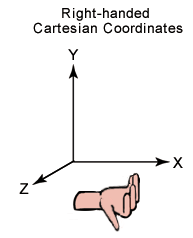
\includegraphics[width=\textwidth]{Bilder/Koordinatensystem.png}
\end{center}\end{column}
\end{columns}
\end{frame}

\subsection{FusionVis - Visualisierungstool}

\begin{frame}\frametitle{Darstellung von Daten im Visualisierungstool}
\begin{center}
	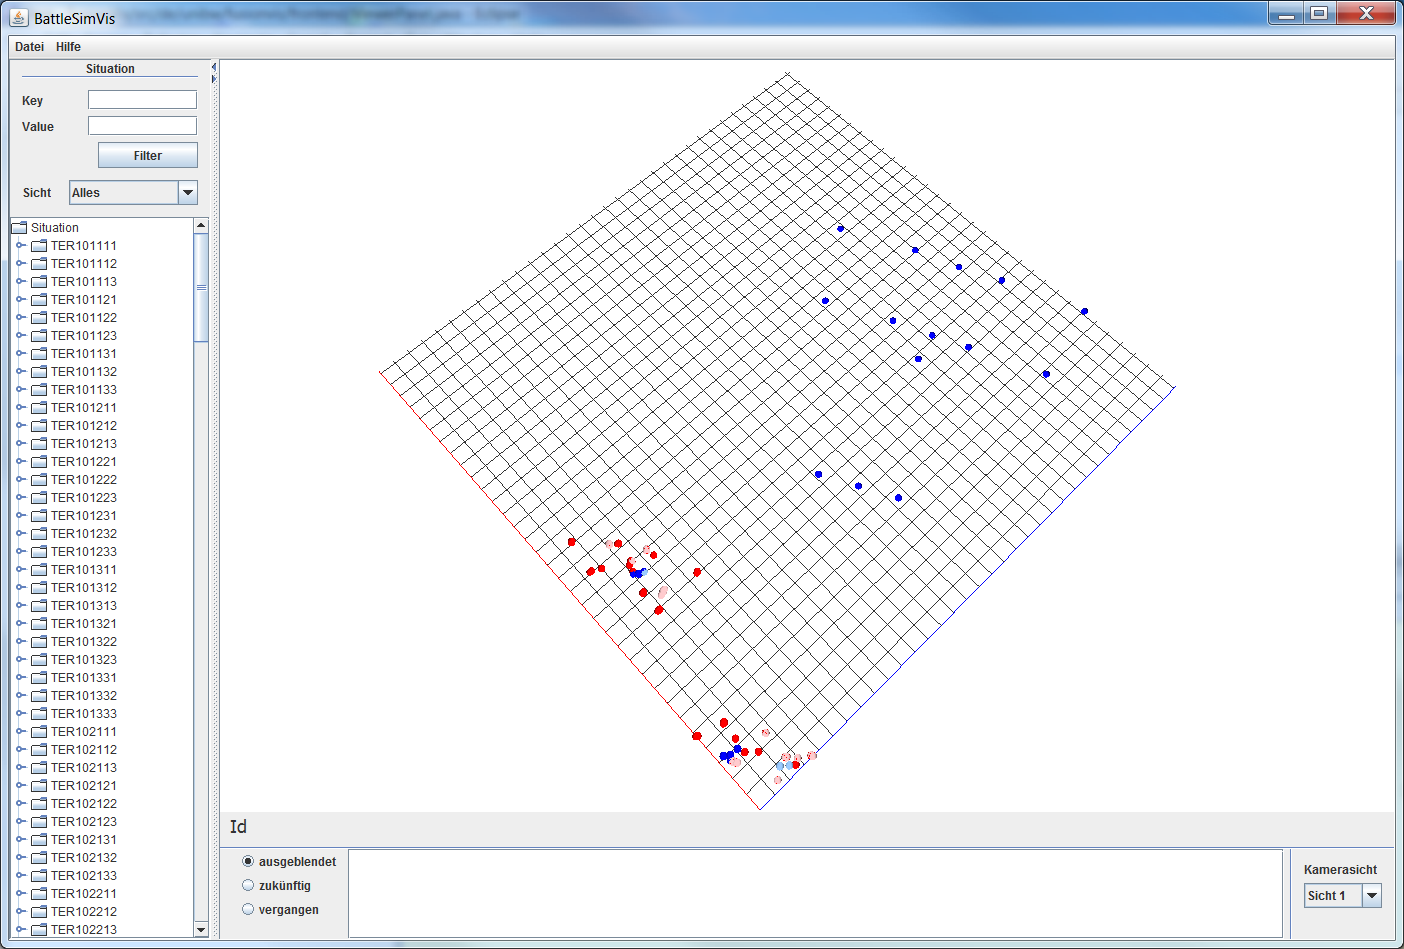
\includegraphics[width=0.7\textwidth]{Bilder/screen.png}
\end{center}
 %   \begin{itemize}
%        \item Freund-/Feind-Unterscheidung
%        \item Unterscheidung beobachtet/real
%        \item Kugel als Datenpunkt
%    \end{itemize}
\end{frame}


\begin{frame}\frametitle{Features}
 \begin{columns}[t]
\begin{column}{5cm}
    \begin{block}{}
    \begin{itemize}
        \item Plattformunabh�ngigkeit
        \item XML-Import
        \item strukturierte textuelle Datendarstellung (Baum)
        \item 3D-Darstellung der Daten
        \item voreingestellte Perspektiven
    \end{itemize}
    \end{block}
\end{column}
\begin{column}{5cm}
    \begin{block}{}
    \begin{itemize}
        \item freie Navigierbarkeit im 3D-Raum
        \item Klassifizierung durch Farben
        \item Datenfilter
        \item Selektion in der 3D-Darstellung
    \end{itemize}
    \end{block}
\end{column}
\end{columns}\end{frame}

\subsection{Fusion}
\begin{frame}\frametitle{Fusion durch Visualisierung}
  \begin{block}{Informationsfusion durch Visualisierung}
   \begin{enumerate}
   	\item ortsgleiche Sichtungen eines Objekts
   	
    \begin{itemize}
	    \item Daten am selben Ort befefinden sich an der selben Stelle
	    \item Ungenauigkeiten (Jitter) k�nnen als solche erkannt werden
     \end{itemize}
   	\item multiple Sichtungen eines Objekts zu unterschiedlichen Zeiten
   	\begin{itemize}
	    \item Annahme: Beobachtete Fahrzeuge haben eine Maximalgeschwindigkeit $v_{max}$
	    \item $v_{max}$ bestimmt die maximale Reichweite in gegebener Zeit
	    \item Reichweite eine Objektes vom Datenpunkt $p_{0}$ aus kann durch ein Volumen $K$ in Form eines Kegels dargestellt werden
	    \item F�r jeden Datenpunkt $p \neq p_{0}$ gilt:\\
	          $p\notin K \rightarrow p \quad ist \quad keine \quad Beobachtung \quad von \quad p_{0}$ 
    \end{itemize}
   \end{enumerate}
\end{block}\end{frame}

\begin{frame}\frametitle{Bewegungstrichter}
\end{frame}


\section{Fazit}

\subsection{Bewertung}
\begin{frame}\frametitle{Bewertung}
\begin{block}{}
  \begin{itemize}[<+-| alert@+>]
  \item Visualisierung erm�glicht Datenfusion
  \item Redundanzen k�nnen reduziert werden
  \item FusionVis als prototypische zeigt die M�glichkeiten
  \item neben dem Prototyp ist ein Visualisierungsframework entstanden
  \item Entwicklungspotential ist vorhanden  
\end{itemize}
 \end{block}
\end{frame}

\subsection{Ausblick}
\begin{frame}\frametitle{Ausblick - Weitere Anwendungsbereiche}
 \begin{block}{NDP - IPv6}
   \begin{itemize}
	  \item Visualisierung von MAC-Adressen, IPv6-Adressen und der Zeit
	  \item Schl�sse �ber verbreitete Hersteller (MAC-Cluster) m�glich
	  \item Auff�lliges Verhalten wird sichtbar 
   \end{itemize}
 \end{block}
 
 \begin{block}{Milit�rische Lagen}
   \begin{itemize}
	  \item Anpassung der Maximalgeschwindigkeiten an Gel�nde und Fahrzeuge
	  \item Kegel verformen sich abh�ngig vom Gel�nde
	  \item genauere Vorhersagen werden m�glich
   \end{itemize}
 \end{block}
\end{frame}


\end{document}